\section{Hardware for Self-driving Cars}
\label{hardware_for_self_driving_cars}

In this chapter, we will discuss sensors, and the various types of them
available for the task of perception. Next we will discuss the self-driving car hardware available nowadays. 

\subsection{Sensors}
\label{sensors}

Let's begin by talking about sensors. Even the best perception algorithms
are limited by the quality of their sensor data. And careful selection of sensors
can go a long way to simplifying the self-driving perception task. Let's try to give a definition of
what a sensor is.


\begin{framed}
\theoremstyle{definition}
\begin{definition}{\textbf{What is a sensor? }}

For our purposes, a sensor is any device that measures or
detects some property of the environment, or changes to that property over time.
\end{definition}
\end{framed}

Sensors are broadly categorized into two types, depending on what property they record. If they record a property of
the environment they are called {\textbf{exteroceptive}}. Extero means outside, or from the surroundings. On the other hand, if the sensors
record a property of the ego vehicle, they are called {\textbf{proprioceptive}}. Proprios means internal, or one's own. Let's start by discussing
common exteroceptive sensors. 

\subsubsection{Camera}

We start with the most common and widely used sensor in autonomous driving, the camera. Cameras are a passive, light-collecting
sensor that are great at capturing rich, detailed information about a scene. In fact, some groups believe that the
camera is the only sensor truly required for self-driving. But state of the art performance is
not yet possible with vision alone. While talking about cameras, we usually tend to talk about three
important comparison metrics. We select cameras in terms:


\begin{itemize}
\item resolution
\item field of view or FOV
\item dynamic range
\end{itemize}

The resolution is the number of pixels that create the image. So it's a way of specifying
the quality of the image.  The field of view is defined by the horizontal and vertical angular extent that is visible to the camera, and can be
varied through lens selection and zoom. The dynamic range of the camera is the difference between the darkest and the lightest tones in an image. High dynamic range is critical for
self-driving vehicles due to the highly variable lighting conditions encountered
while driving especially at night. 

There is an important trade off cameras and lens selection, that lies between the choice of
field of view and resolution. Wider FOV permits a lager
viewing region in the environment, but fewer pixels that absorb light from one particular object. As the FOV increases, we need to increase resolution to still be
able to perceive with the same quality, the various kinds of information we may encounter. 
Other properties of cameras that affect perception exist as well, such as focal length, depth of field and frame rate. 
 
The combination of two cameras with overlapping fields of view and aligned image planes is
called the stereo camera. Stereo cameras allow depth estimation
from synchronized image pairs. Pixel values from image can be
matched to the other image producing a disparity map of the scene. This disparity can then be used
to estimate depth at each pixel. 

\subsubsection{LIDAR}

Next we have LIDAR which stands for light detection and ranging sensor. LIDAR sensing involves shooting
light beams into the environment and measuring the reflected return. By measuring the amount of returned
light and time of flight of the beam. Both in intensity in range to
the reflecting object can be estimated. An illustration of LIDAR based environment representation is shown in figure \ref{lidar_illustrate}.

\begin{figure}[!htb]
\begin{center}
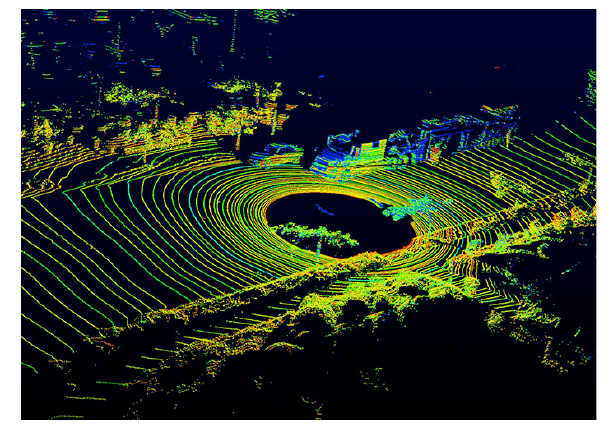
\includegraphics[scale=0.280]{img/hardware/lidar_illustrate.jpeg}
\end{center}
\caption{LIDAR illustration of environment representation.}
\label{lidar_illustrate}
\end{figure}

LIDAR usually includes a spinning element
with multiple stacked light sources and outputs a three dimensional
point cloud map, which is great for assessing scene geometry. Because it is an active sensor
with it's own light sources, LIDAR are not effected by
the environments lighting. So LIDAR do not face the same challenges
as cameras when operating in poor or variable lighting conditions. Let's discuss the important comparison
metrics for selecting LIDAR.

\begin{itemize}
\item The first is the number of sources it contains with 8, 16, 32, and 64 being common sizes. 
\item the second is the points per second it can collect. The faster the point collection, the more
detailed the 3D point cloud can be. 
\end{itemize}

Another characteristic is the rotation rate. The higher this rate, the faster
the 3D point clouds are updated. Detection range is also important, and is dictated by the power
output of the light source. And finally, we have the field of view,
which once again, is the angular extent
visible to the LIDAR sensor. 

Finally, we should also mention the new
LIDAR types that are currently emerging. High-resolution, solid-state LIDAR. Without a rotational component
of the typical LIDARs, these sensors stand to become
extremely low-cost and reliable. Thanks to being implemented
entirely in silicon. HD solid-state LIDAR
are still a work in progress. But definitely something exciting for
the future of affordable self-driving. 

\subsubsection{Radar}

Our next sensor is RADAR, which stands for radio detection and ranging. RADAR sensors have been
around longer than LIDAR and robustly detect large objects in the environment. They are particularly useful in adverse
weather as they are mostly unaffected by precipitation. Let's discuss some of the comparison
metrics for selecting RADAR. RADAR are selected based on

\begin{itemize}
\item detection range
\item field of view, 
\item the position and speed measurement accuracy. 
\end{itemize}

RADARs are also typically available as either having a wide angular field of view but short range. 
Or having a narrow FOV but a longer range. 


\subsubsection{Ultrasonics or sonars}

The next sensor we are going to discuss are ultrasonics or sonars. Originally so named for
sound navigation and ranging. Which measure range using sound waves. Sonars are sensors that are short
range and inexpensive ranging devices. This makes them good for parking scenarios, where the ego-vehicle needs to make
movements very close to other cars. Another great thing about sonar is that they are low-cost. Moreover, just like RADAR and LIDAR,
they are unaffected by lighting and precipitation conditions. A sonar sensor is selected based
on a few key metrics itemized next. 

\begin{itemize}
\item The maximum range they can measure
\item The the detection FOV
\item The cost
\end{itemize}

\subsubsection{Proprioceptive sensors}

Now let's discuss the proprioceptive sensors, the sensors that sense ego properties. The most common ones here
are:

\begin{itemize}
\item Global Navigation Satellite Systems, GNSS for short, such as GPS or Galileo
\item Inertial Measurement Units or IMU's
\item Wheel odometers
\end{itemize}

GNSS receivers are used to measure ego vehicle position, velocity, and sometimes heading. The accuracy depends a lot on
the actual positioning methods and the corrections used. Apart from these, the IMU also
measures the angular rotation rate, accelerations of the ego vehicle, and
the combined measurements can be used to estimate the 3D orientation
of the vehicle. Where heading is the most important for
vehicle control. Finally, we have wheel odometry sensors. This sensor tracks the wheel
rates of rotation, and uses these to estimate the speed and
heading rate of change of the ego car. This is the same sensor that tracks
the mileage on your vehicle. 

In summary, the major sensors used nowadays for autonomous driving perception
include cameras, RADAR, LIDAR, sonar, GNSS, IMUs,
and wheel odometry modules. These sensors have many characteristics that can vary wildly, including resolution,
detection range, and FOV. 

Selecting an appropriate sensor configuration for a self-driving car is not trivial. Figure \ref{sensors_positioning} is a simple graphic that
shows each of the sensors and where they usually go on a car. 

\begin{figure}[!htb]
\begin{center}
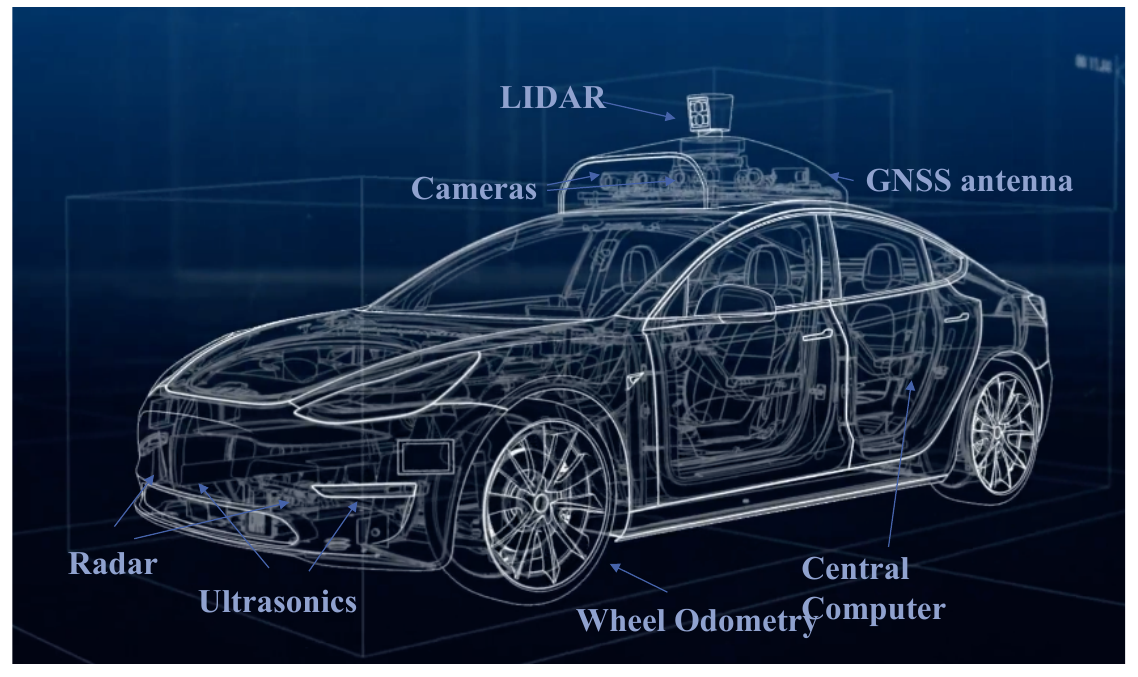
\includegraphics[scale=0.280]{img/hardware/sensors_positioning.jpeg}
\end{center}
\caption{Usual sensor positioning.}
\label{sensors_positioning}
\end{figure}


\subsection{Computing Hardware}
\label{computing_hardware}

Let's now discuss a little bit about the computing hardware most commonly used in  self-driving cars at the time of writing. The most crucial part
is the computing brain, the main decision making unit of the car. It takes in all sensor data and outputs
the commands needed to drive the vehicle. Most companies prefer to design their own
computing systems that match the specific requirements of their sensors and
algorithms. Some hardware options exist, however, that can handle self-driving computing loads out of the box. 

The most common examples would be Nvidia's Drive PX and Intel \& Mobileye's EyeQ. Any computing brain for self-driving needs
both serial and parallel compute modules. Particularly for image and LIDAR processing to do segmentation, object detection, and mapping. 
For these we employ GPUs, FPGAs and custom ASICs (Application Specific Integrated Circuit), which are specialized hardware to
do a specific type of computation. 

For example, the drive PX units include multiple GPUs. The EyeQs have FPGAs both to
accelerate parallalizable compute tasks, such as image processing or
neural network inference. 

Finally, a quick comment about synchronization. Because we want to make driving
decisions based on a coherent picture of the road scene. It is essential to correctly synchronize
the different modules in the system, and serve a common clock. Fortunately, GPS relies on extremely
accurate timing to function, and as such can act as an appropriate
reference clock when available. Regardless, sensor measurements must be
timestamped with consistent times for sensor fusion to function correctly. Let's summarize. In this video,
we learned about sensors and their different types based
on what they measure. 

\subsection{Hardware Configuration}
\label{hardware_configuration}

Section \ref{sensors}, covers the various kinds of sensors most commonly used for perception. 
One question that should be answered is how do we place these sensors on the vehicle in order to  aquire a complete view of the environment? 


In this section, we will discuss the configuration design to meet sensor coverage needs for an autonomous driving car. 
We will do this by going through two common scenarios:

\begin{itemize}
\item Driving on a highway and 
\item Driving in an urban environment
\end{itemize}
 
After analyzing these scenarios, we will lay out the overall coverage requirements and discuss some issues with the design. 

Let's however begin by recalling the most commonly available sensors. These are:

\begin{itemize}
\item The camera for appearance input. 
\item The stereo camera for depth information
\item Lidar for all whether 3D input
\item Radar for object detection
\item Ultrasonic for short-range 3D input 
\item GNSS/IMU data and wheel odometry for ego state estimation. 
\end{itemize}

Also, remember that all of these sensors come in different configurations and  different ranges in FOV over which they can sense. 
They have some resolution that depends on the instrument specifics and the field of view. Before we move to discussing coverage, let's define the deceleration rates we're willing to accept for driving which will drive the detection ranges needed for our sensors. 


\begin{framed}
\theoremstyle{remark}
\begin{remark}{\textbf{Aggressive Deceleration}}

Aggressive deceleration is set to $5 m/sec^2$ which is roughly the deceleration you experience when you slam the brakes hard and try to stop abruptly in case of an emergency. 
\end{remark}
\end{framed}

Normal decelerations are set to $2 m/sec^2$, which is reasonably comfortable while still allowing the car to come to a stop quickly. 
Given a constant deceleration our braking distance $d$ can be computed as follows according to equation \ref{stopping_distance}.

\begin{equation}
d = \frac{V^2}{2\alpha}
\label{stopping_distance}
\end{equation}

where $V$ is the vehicle velocity and  $\alpha$ is its rate of deceleration. 
We can also factor in reaction time of the system and road surface friction limits, but we'll keep things simple in this discussion. 

Let's talk about coverage now. The question we want to answer is where should we place our sensors so that we have sufficient input for our driving task? 
Practically speaking, we want our sensors to capture the ODD we have in mind or the ODD our system can produce decisions for. 
We should be able to provide all of the decisions with sufficient input. 
There can be so many possible scenarios in driving but we'll look at just two common scenarios to see how the requirements drive our sensor selection. 
Will look at highway and urban driving. Let's think about these two situations briefly. 


For a divided highway, we have fast moving traffic, usually high volume, and quite a few lanes to monitor, 
but all vehicles are moving in the same direction. The other highlight of driving on a highway setting is that there are 
fewer and gradual curves and we have exits and merges to consider as well. 

On the other hand, in the urban situation we'll consider, 
we have moderate volume and moderate speed traffic with fewer lanes but with 
traffic moving in all directions especially through intersections. 

\subsubsection{Highway Scenario}

Let's start with the highway setting. 
We can break down the highway setting into three basic maneuver needs. 

\begin{itemize}
\item We may need to hit the brakes hard if there's an emergency situation. 
\item We need to maintain a steady speed matching the flow of traffic around us.
\item We might need to change lanes. 
\end{itemize}

In the case of an emergency stop, if there is a blockage on our road we want to stop in time. 
So, applying our stopping distance equation longitudinally, we need to be able to sense about a 110 meters in front of us assuming a highway speed of a 120 kilometers and aggressive deceleration. 
Most self-driving systems aim for sensing ranges of a 150 to 200 meters in front of the vehicle as a result. 
Similarly, to avoid lateral collision or to change lanes to avoid hitting an obstacle in our lane, we need to be able to sense at least our adjacent lanes, 
which are 3.7 meters wide in North America. To maintain speed during vehicle following, we need to sense the vehicle in our own lane. 
Both their relative position and the speed are important to maintain a safe following distance. 
This is usually defined in units of time for human drivers and set to two seconds in nominal conditions. 
It can also be assessed using aggressive deceleration of the lead vehicle and the reaction time from our ego vehicle. 
So, at a 120 kilometers per hour, relative position and speed measurements to a range of 165 meters are needed and typical systems use 100 meters for this requirement. 
Laterally, we need to know what's happening anywhere in our adjacent lanes in case another vehicles seeks to merge into our lane or we need to merge with other traffic. 
A wide 160 to 180 degree field of view is required to track adjacent lanes and a range of 40 to 60 meters is needed to find space between vehicles. 

Finally, let's discuss the lane change maneuver and consider the following scenario. 
Suppose we want to move to the adjacent lane, longitudinally we need to look forward, so we are a safe distance from the leading vehicle and 
we also need to look behind just to see what the rear vehicles are doing and laterally it's a bit more complicated. 
We may need to look beyond just the adjacent lanes. For example, what if a vehicle attempts to maneuver into the adjacent lane at the same time as we do? 
We'll need to coordinate our lane change room maneuvers so we don't crash. 

The sensor requirements for lane changes are roughly equivalent to those in the maintain speed scenario. 
As both need to manage vehicles in front of and behind the ego vehicle as well as to each side. 
Overall, this gives us the picture for coverage requirements for the highway driving scenario. 
We need longitudinal sensors and lateral sensors and both wide and narrow FOV sensors to do these three maneuvers, the emergency stop, maintaining speed and changing lanes. 
Already from this small set of ODD requirements we see a large variety of sensor requirements that arise. 


\begin{figure}[!htb]
\begin{center}
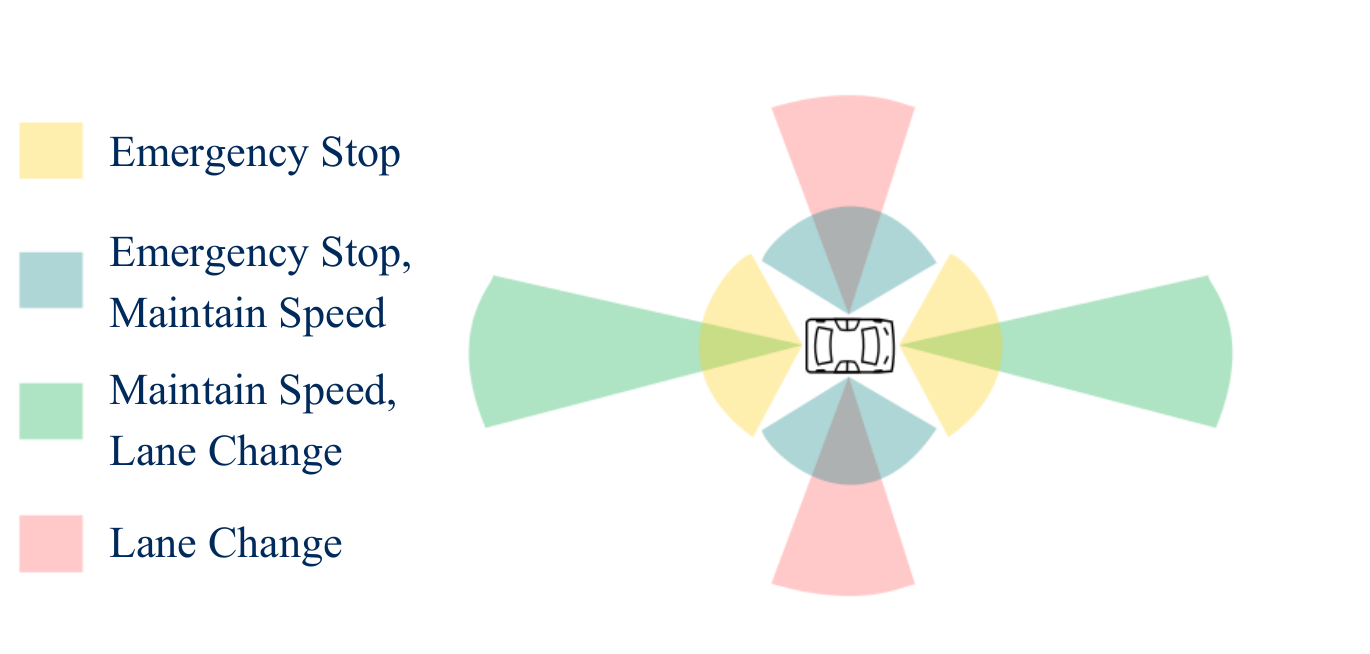
\includegraphics[scale=0.280]{img/hardware/highway_analysis_overall_coverage.jpeg}
\end{center}
\caption{Highway analysis overall coverage.}
\label{highway_analysis_overall_coverage}
\end{figure}

\subsubsection{Urban Scenario}
\label{urban_scenario}

Let's discuss the urban scenario next. 
The urban scenario as we discussed before is a moderate volume, moderate traffic scenario with fewer lanes on the highway case but with the added complexity of pedestrians. 
There are six types of basic maneuvers here. Obviously, we can still perform emergency stop, maintain speed and lane changes but we also have scenarios such as overtaking a parked car, 
left and right turns at intersections and more complex maneuvers through intersections such as roundabouts. 
In fact, for the first three basic maneuvers, the coverage analysis is pretty much the same as the highway analysis but since we are not moving as quickly, 
we don't need the same extent for our long-range sensing. 

Let's discuss the overtake maneuver next. 
More specifically, consider a case where you have to overtake a parked car. 
Longitudinally, we definitely need to sense the parked car as well as look for oncoming traffic. 
So, we need both sensors, wide short-range sensors to detect the parked car and narrow long-range sensors to identify if oncoming traffic is approaching. 
Laterally, we'll need to observe beyond the adjacent lanes for merging vehicles as we did in the highway case. 
Intersections require that  we  have near omni-directional sensing for all kinds of movements that can occur. 
Approaching vehicles, nearby pedestrians, doing turns and much more. 
Finally, for roundabouts we need a wide-range, short distance sensor laterally since the traffic is slow but 
we also need a wide-range short distance sensor longitudinally because of how movement around the roundabout occurs. 
We need to sense all of the incoming traffic flowing through the roundabout to make proper decisions. 

Thus, we end up with the overall coverage diagram for the urban case shown in figure \ref{urban_analysis_overall_coverage}. 
The main difference with respect to highway coverage is because of the sensing we require 
for movement at intersections and at roundabouts and for the overtaking maneuver. 
In fact, the highway case is almost entirely covered by the urban requirements. 


\begin{figure}[!htb]
\begin{center}
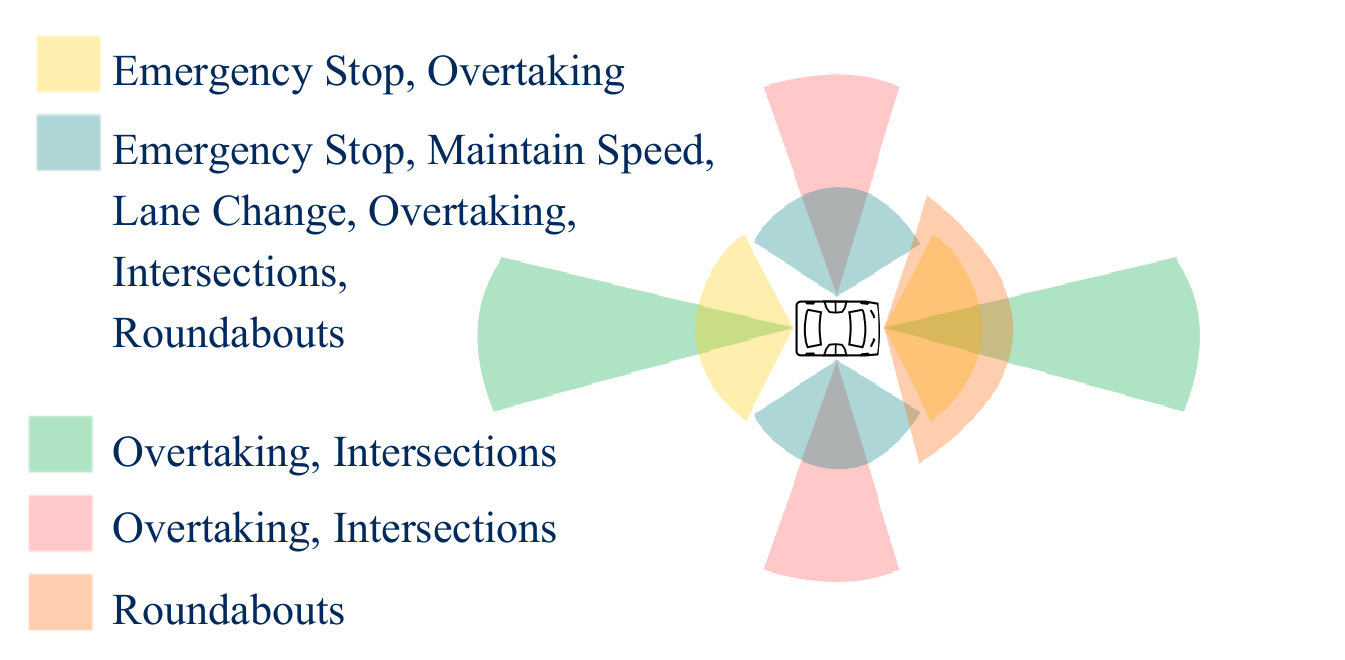
\includegraphics[scale=0.280]{img/hardware/urban_analysis_overall_coverage.jpeg}
\end{center}
\caption{Urban analysis overall coverage.}
\label{urban_analysis_overall_coverage}
\end{figure}


Let's summarize the coverage analysis. For all of the maneuvers we do, we need long range sensors which typically 
have shorter angular field of view and wide angular field of view sensors which typically have medium to short-range sensing. 
As the scenarios become more complex, we saw the need for full 360 degrees sensor coverage on the short scale out to 
about 50 meters and much longer range requirements in the longitudinal direction. 
We can also add even shorter range sensors like sonar which are useful in parking scenarios and so in the end our sensor configuration looks something like this diagram. 


\begin{figure}[!htb]
\begin{center}
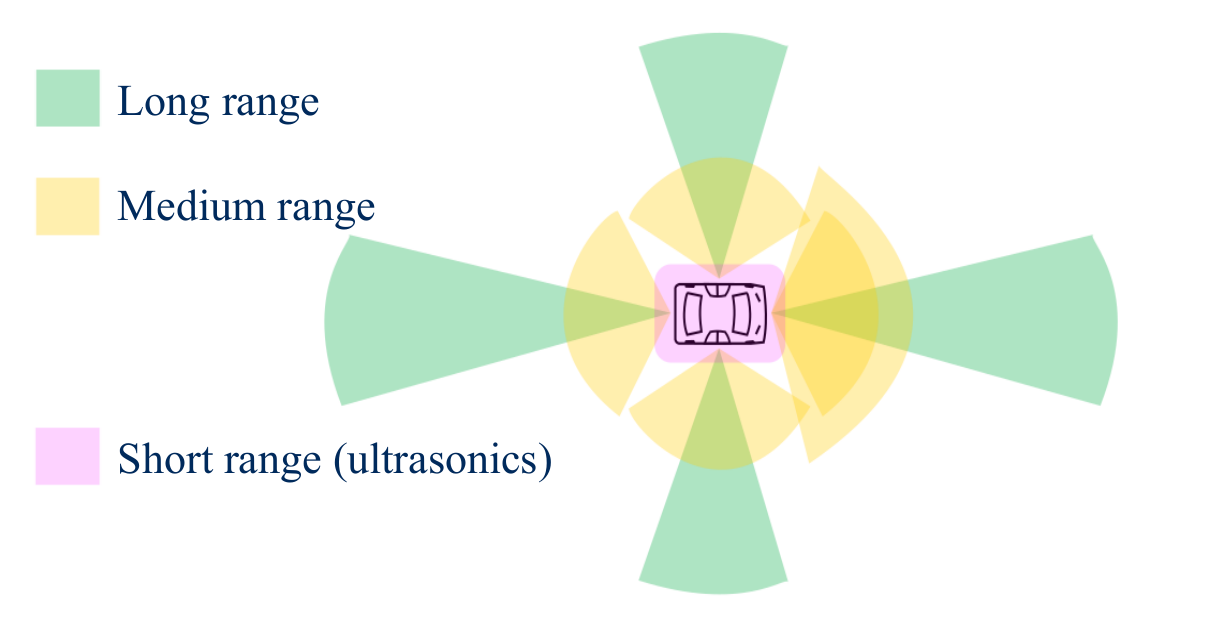
\includegraphics[scale=0.280]{img/hardware/overall_coverage.jpeg}
\end{center}
\caption{Overall coverage.}
\label{overall_coverage}
\end{figure}


To summarize, our choice of sensors should be driven by the requirements of the maneuvers we want to execute and it should include 
both long-range sensors for longitudinal dangers and wide field of view sensors for omnidirectional perception. 
The final choice of configurations also depends on our requirements for operating conditions, sensor redundancy due to failures and on budget. 
There is no single answer to which sensors are needed for a self-driving car. 


